%%%%%%%%%%%%%%%%%%%%%%%%%%%%%%%%%%%%%%%%%
% Programming/Coding Assignment
% LaTeX Template
%
% This template has been downloaded from:
% http://www.latextemplates.com
%
% Original author:
% Ted Pavlic (http://www.tedpavlic.com)
%
% Note:
% The \lipsum[#] commands throughout this template generate dummy text
% to fill the template out. These commands should all be removed when 
% writing assignment content.
%
% This template uses a Perl script as an example snippet of code, most other
% languages are also usable. Configure them in the "CODE INCLUSION 
% CONFIGURATION" section.
%
%%%%%%%%%%%%%%%%%%%%%%%%%%%%%%%%%%%%%%%%%

%----------------------------------------------------------------------------------------
%	PACKAGES AND OTHER DOCUMENT CONFIGURATIONS
%----------------------------------------------------------------------------------------

\documentclass[a4paper]{article}

\usepackage{fancyhdr} % Required for custom headers
\usepackage{lastpage} % Required to determine the last page for the footer
\usepackage{extramarks} % Required for headers and footers
\usepackage[usenames,dvipsnames]{color} % Required for custom colors
\usepackage{graphicx} % Required to insert images
\usepackage{listings} % Required for insertion of code
\usepackage{courier} % Required for the courier font
\usepackage{lipsum} % Used for inserting dummy 'Lorem ipsum' text into the template
\usepackage{multirow}
\usepackage{tabu}
\usepackage{float}
\usepackage{pbox}
\usepackage{subcaption}
\usepackage{algpseudocode}

\usepackage{listings}
\usepackage{color}

\definecolor{dkgreen}{rgb}{0,0.6,0}
\definecolor{gray}{rgb}{0.5,0.5,0.5}
\definecolor{mauve}{rgb}{0.58,0,0.82}

\lstset{frame=tb,
  language=Matlab,
  aboveskip=3mm,
  belowskip=3mm,
  showstringspaces=false,
  columns=flexible,
  basicstyle={\small\ttfamily},
  numbers=none,
  numberstyle=\tiny\color{gray},
  keywordstyle=\color{blue},
  commentstyle=\color{dkgreen},
  stringstyle=\color{mauve},
  breaklines=true,
  breakatwhitespace=true
  tabsize=3
}

% Margins
\topmargin=-0.45in
\evensidemargin=0in
\oddsidemargin=0in
\textwidth=6.5in
\textheight=9.5in
\headsep=0.25in

\linespread{1.1} % Line spacing

% Set up the header and footer
\pagestyle{fancy}
\lhead{\hmwkAuthorName} % Top left header
\chead{\hmwkShortTitle} % Top center head
\rhead{\firstxmark} % Top right header
\lfoot{\lastxmark} % Bottom left footer
\cfoot{} % Bottom center footer
\rfoot{Page\ \thepage\ of\ \protect\pageref{LastPage}} % Bottom right footer
\renewcommand\headrulewidth{0.4pt} % Size of the header rule
\renewcommand\footrulewidth{0.4pt} % Size of the footer rule

\setlength\parindent{0pt} % Removes all indentation from paragraphs

%----------------------------------------------------------------------------------------
%	CODE INCLUSION CONFIGURATION
%----------------------------------------------------------------------------------------

\definecolor{MyDarkGreen}{rgb}{0.0,0.4,0.0} % This is the color used for comments
\lstloadlanguages{Matlab} % Load Perl syntax for listings, for a list of other languages supported see: ftp://ftp.tex.ac.uk/tex-archive/macros/latex/contrib/listings/listings.pdf
\lstset{language=Matlab, % Use Perl in this example
        frame=single, % Single frame around code
        basicstyle=\small\ttfamily, % Use small true type font
        keywordstyle=[1]\color{Blue}\bf, % Perl functions bold and blue
        keywordstyle=[2]\color{Purple}, % Perl function arguments purple
        keywordstyle=[3]\color{Blue}\underbar, % Custom functions underlined and blue
        identifierstyle=, % Nothing special about identifiers                                         
        commentstyle=\usefont{T1}{pcr}{m}{sl}\color{MyDarkGreen}\small, % Comments small dark green courier font
        stringstyle=\color{Purple}, % Strings are purple
        showstringspaces=false, % Don't put marks in string spaces
        tabsize=5, % 5 spaces per tab
        %
        % Put standard Perl functions not included in the default language here
        morekeywords={rand},
        %
        % Put Perl function parameters here
        morekeywords=[2]{on, off, interp},
        %
        % Put user defined functions here
        morekeywords=[3]{test},
       	%
        morecomment=[l][\color{Blue}]{...}, % Line continuation (...) like blue comment
        numbers=left, % Line numbers on left
        firstnumber=1, % Line numbers start with line 1
        numberstyle=\tiny\color{Blue}, % Line numbers are blue and small
        stepnumber=5 % Line numbers go in steps of 5
}

% Creates a new command to include a perl script, the first parameter is the filename of the script (without .pl), the second parameter is the caption
\newcommand{\matlabscript}[2]{
\begin{itemize}
\item[]\lstinputlisting[caption=#2,label=#1]{#1.m}
\end{itemize}
}

%----------------------------------------------------------------------------------------
%	DOCUMENT STRUCTURE COMMANDS
%	Skip this unless you know what you're doing
%----------------------------------------------------------------------------------------

% Header and footer for when a page split occurs within a problem environment
\newcommand{\enterProblemHeader}[1]{
\nobreak\extramarks{#1}{#1 continued on next page\ldots}\nobreak
\nobreak\extramarks{#1 (continued)}{#1 continued on next page\ldots}\nobreak
}

% Header and footer for when a page split occurs between problem environments
\newcommand{\exitProblemHeader}[1]{
\nobreak\extramarks{#1 (continued)}{#1 continued on next page\ldots}\nobreak
\nobreak\extramarks{#1}{}\nobreak
}

\setcounter{secnumdepth}{0} % Removes default section numbers
\newcounter{homeworkProblemCounter} % Creates a counter to keep track of the number of problems

\newcommand{\homeworkProblemName}{}
\newenvironment{homeworkProblem}[1][Problem \arabic{homeworkProblemCounter}]{ % Makes a new environment called homeworkProblem which takes 1 argument (custom name) but the default is "Problem #"
\stepcounter{homeworkProblemCounter} % Increase counter for number of problems
\renewcommand{\homeworkProblemName}{#1} % Assign \homeworkProblemName the name of the problem
\section{\homeworkProblemName} % Make a section in the document with the custom problem count
\enterProblemHeader{\homeworkProblemName} % Header and footer within the environment
}{
\exitProblemHeader{\homeworkProblemName} % Header and footer after the environment
}

\newcommand{\problemAnswer}[1]{ % Defines the problem answer command with the content as the only argument
\noindent\framebox[\columnwidth][c]{\begin{minipage}{0.98\columnwidth}#1\end{minipage}} % Makes the box around the problem answer and puts the content inside
}

\newcommand{\homeworkSectionName}{}
\newenvironment{homeworkSection}[1]{ % New environment for sections within homework problems, takes 1 argument - the name of the section
\renewcommand{\homeworkSectionName}{#1} % Assign \homeworkSectionName to the name of the section from the environment argument
\subsection{\homeworkSectionName} % Make a subsection with the custom name of the subsection
\enterProblemHeader{\homeworkProblemName\ [\homeworkSectionName]} % Header and footer within the environment
}{
\enterProblemHeader{\homeworkProblemName} % Header and footer after the environment
}

%----------------------------------------------------------------------------------------
%	NAME AND CLASS SECTION
%----------------------------------------------------------------------------------------

\newcommand{\hmwkTitle}{CO395 Machine Learning\\CBC \#3\\Case Based Reasoning} % Assignment title
\newcommand{\hmwkShortTitle}{CBC \#3 - Case Based Reasoning}
\newcommand{\hmwkDueDate}{Monday,\ November\ 4,\ 2013} % Due date
\newcommand{\hmwkAuthorName}{Group 1} % Your name

%----------------------------------------------------------------------------------------
%	TITLE PAGE
%----------------------------------------------------------------------------------------

\title{
\vspace{2in}
\textmd{\textbf{\hmwkTitle}}\\
%\normalsize\vspace{0.1in}\small{Due\ on\ \hmwkDueDate}\\
%\vspace{0.1in}\large{\textit{\hmwkClassInstructor\ \hmwkClassTime}}
\vspace{3in}
\textbf{Group 1}\\
Yong Wen Chua, \texttt{ywc110}\\
Thomas Morrison, \texttt{tm1810}\\
Marcin Baginski, \texttt{mgb10}\\
Marcin Kadziela, \texttt{mk4910}
}

%\author{\textbf{\hmwkAuthorName}}

\date{} % Insert date here if you want it to appear below your name

%----------------------------------------------------------------------------------------

\begin{document}

\maketitle

%----------------------------------------------------------------------------------------
%	TABLE OF CONTENTS
%----------------------------------------------------------------------------------------

%\setcounter{tocdepth}{1} % Uncomment this line if you don't want subsections listed in the ToC

\newpage
\tableofcontents
\newpage

%----------------------------------------------------------------------------------------
%	SECTION 1 - Implementation Details
%----------------------------------------------------------------------------------------

\section{Implementation Details}

\subsection{Overview}
We implemented a case as a MATLAB struct with the following fields:
\begin{itemize} \itemsep0pt \parskip0pt \parsep0pt
\item \texttt{au} - which represents the AUs which are active
\item \texttt{class} - which represents the emotion (can be 0 for a case which does not have a solution yet)
\item \texttt{typicality} - which represents the number of times this exact case has been encountered during training and subsequently during the RETAIN phase
\end{itemize}
Our Case Base is a column vector where each cell represents a case. \medskip

\subsection{Description of the MATLAB functions}
\begin{itemize}
\item \texttt{CBRInit(x,y)} - this function initialises the case base. It takes as arguments the examples \texttt{x} and classifications \texttt{y} and returns the case base in the format described in the previous subsection
\item \texttt{retrieve(cbr, newCase)} - this function implements a modified version of the k-NN algorithm to return a set of cases which closest match the \texttt{newCase}. Along with the cases, the function reports a distance from each returned case to the \texttt{newCase}. The modification of the original k-NN algorithm comes from the fact, that if at least two largest distances returned from the function are equal, the function returns \texttt{k+n} cases such that \texttt{n} is the smallest natural number which makes sure that no case which have the distance equal to the largest one in the original \texttt{k} cases is omitted. This modification is useful because in situations where there are more than \texttt{k} cases with the same distance to the \texttt{newCase}, we do not want to restrict ourselves to considering only the ones, which appear first in our case base. We implemented the Manhattan and Euclidean distances as our similarity measures.
\item \texttt{reuse(cases, newCase)} - this function takes as arguments the cases returned by the \texttt{retrieve} function as well as the new case without a solution. It performs the majority-voting weighted by the distance of the existing \texttt{cases} in order to determine the most probable solution to the \texttt{newCase}. If there are two or more emotions which have the equal number of 'votes', then the preferred 'vote' is given to the case with a higer value in the \texttt{typicality} field. If there is still ambiguity even after this step, the function removes one of the existing \texttt{cases} which has the largest distance and repeats all the steps. The algorithm will terminate in the worst-case scenario when it will be left with just a single case
\item \texttt{retain(cbr, newCase)} - this function updates the Case Base with the new case. If the new case does not already exist in the case base, it simply appends it at the end. Otherwise, it increments the \texttt{typicality} field in an identical, existing case
\item \texttt{makeCase(AUs, class)} - creates a single case struct as described above. It can take either of the two representations of the active AUs as an argument
\item \texttt{nFoldValidate(examples, classifications, n)} - preforms the n-fold cross-validation and returns the confusion matrices for each fold
\item \texttt{testCBR(cbr,x2)} - takes the Case Base and a matrix of examples to be classified and returns a column vector of predictions
\end{itemize}
\clearpage

%----------------------------------------------------------------------------------------
%	SECTION 2 - Evaluation
%----------------------------------------------------------------------------------------

\section{Evaluation}
The results presented in this section are for the modified (as explained in the Implementation Details) distance-weighted \textbf{5-NN} algorithm on the \emph{clean} dataset and \textbf{9-NN} on the \emph{noisy} one. We chose these algorithms because they performed best during our tests. Other variations of the algorithm are analysed in the next section under 'Comparison of similarity measures'.

\subsection{Clean dataset}

\begin{table}[H]
\center
\begin{tabu}{cc|c|c|c|c|c|c|}
\cline{3-8}
& & \multicolumn{6}{ c| }{Predicted class} \\ \cline{3-8}
& & 1 & 2 & 3 & 4 & 5 & 6 \\ \cline{1-2} \tabucline[1.5pt]{3-8}
\multicolumn{1}{ |c| }{\multirow{6}{*}{Actual class} } &
\multicolumn{1}{ |c|[1.5pt] }{1} & \textbf{97} & 18 & 4 & 4 & 8 & 1 \\ \cline{2-8}
\multicolumn{1}{ |c| }{}                        &
\multicolumn{1}{ |c|[1.5pt] }{2} & 7 & \textbf{178} & 1 & 6 & 5 & 1 \\ \cline{2-8}
\multicolumn{1}{ |c|  }{}                        &
\multicolumn{1}{ |c|[1.5pt] }{3} & 3 & 3 & \textbf{96} & 0 & 2 & 15 \\ \cline{2-8}
\multicolumn{1}{ |c|  }{}                        &
\multicolumn{1}{ |c|[1.5pt] }{4} & 0 & 6 & 1 & \textbf{207} & 0 & 2 \\ \cline{2-8}
\multicolumn{1}{ |c|  }{}                        &
\multicolumn{1}{ |c|[1.5pt] }{5} & 4 & 16 & 2 & 5 & \textbf{103} & 2 \\ \cline{2-8}
\multicolumn{1}{ |c|  }{}                        &
\multicolumn{1}{ |c|[1.5pt] }{6} & 1 & 1 & 6 & 6 & 0 & \textbf{193} \\ \cline{1-8}
\end{tabu}
\caption{Confusion Matrix for the modified 5-NN distance-weighted algorithm on the \emph{clean} dataset}
\label{confusionMatrixClean5NN}
\end{table}

\begin{table}[H]
\center
\begin{tabu}{cc|c|c|c|}
\cline{3-5}
& & Recall & Precision & $F_1$ \\ \cline{1-2} \tabucline[1.5pt]{3-5}
\multicolumn{1}{ |c| }{\multirow{6}{*}{Actual class} } &
\multicolumn{1}{ |c|[1.5pt] }{1} & 73\% & 87\% & 80\% \\ \cline{2-5}
\multicolumn{1}{ |c| }{}                        &
\multicolumn{1}{ |c|[1.5pt] }{2} & 90\% & 80\% & 85\% \\ \cline{2-5}
\multicolumn{1}{ |c|  }{}                        &
\multicolumn{1}{ |c|[1.5pt] }{3} & 81\% & 87\% & 84\% \\ \cline{2-5}
\multicolumn{1}{ |c|  }{}                        &
\multicolumn{1}{ |c|[1.5pt] }{4} & 96\% & 91\% & 93\% \\ \cline{2-5}
\multicolumn{1}{ |c|  }{}                        &
\multicolumn{1}{ |c|[1.5pt] }{5} & 78\% & 87\% & 82\% \\ \cline{2-5}
\multicolumn{1}{ |c|  }{}                        &
\multicolumn{1}{ |c|[1.5pt] }{6} & 93\% & 90\% & 92\% \\ \cline{1-5}
\end{tabu}
\caption{Recall, precision and $F_1$ measure for the modified 5-NN distance-weighted algorithm on the \emph{clean} dataset}
\label{recallPrecisionF1Clean5NN}
\end{table}

\begin{figure}[H]
\[ C = \frac{874}{1004} = 87.1\% \]
\caption{Classification rate for the modified 5-NN distance-weighted algorithm on the \emph{clean} dataset}
\end{figure}

\subsection{Noisy dataset}

\begin{table}[H]
\center
\begin{tabu}{cc|c|c|c|c|c|c|}
\cline{3-8}
& & \multicolumn{6}{ c| }{Predicted class} \\ \cline{3-8}
& & 1 & 2 & 3 & 4 & 5 & 6 \\ \cline{1-2} \tabucline[1.5pt]{3-8}
\multicolumn{1}{ |c| }{\multirow{6}{*}{Actual class} } &
\multicolumn{1}{ |c|[1.5pt] }{1} & \textbf{15} & 11 & 31 & 4 & 22 & 5 \\ \cline{2-8}
\multicolumn{1}{ |c| }{}                        &
\multicolumn{1}{ |c|[1.5pt] }{2} & 0 & \textbf{160} & 15 & 3 & 6 & 3 \\ \cline{2-8}
\multicolumn{1}{ |c|  }{}                        &
\multicolumn{1}{ |c|[1.5pt] }{3} & 4 & 10 & \textbf{133} & 9 & 6 & 25 \\ \cline{2-8}
\multicolumn{1}{ |c|  }{}                        &
\multicolumn{1}{ |c|[1.5pt] }{4} & 3 & 8 & 11 & \textbf{170} & 4 & 13 \\ \cline{2-8}
\multicolumn{1}{ |c|  }{}                        &
\multicolumn{1}{ |c|[1.5pt] }{5} & 5 & 5 & 14 & 2 & \textbf{74} & 10 \\ \cline{2-8}
\multicolumn{1}{ |c|  }{}                        &
\multicolumn{1}{ |c|[1.5pt] }{6} & 1 & 1 & 8 & 7 & 9 & \textbf{194} \\ \cline{1-8}
\end{tabu}
\caption{Confusion Matrix for the modified 9-NN distance-weighted algorithm on the \emph{noisy} dataset}
\label{confusionMatrixNoisy9NN}
\end{table}

\begin{table}[H]
\center
\begin{tabu}{cc|c|c|c|}
\cline{3-5}
& & Recall & Precision & $F_1$ \\ \cline{1-2} \tabucline[1.5pt]{3-5}
\multicolumn{1}{ |c| }{\multirow{6}{*}{Actual class} } &
\multicolumn{1}{ |c|[1.5pt] }{1} & 17\% & 54\% & 26\% \\ \cline{2-5}
\multicolumn{1}{ |c| }{}                        &
\multicolumn{1}{ |c|[1.5pt] }{2} & 86\% & 82\% & 84\% \\ \cline{2-5}
\multicolumn{1}{ |c|  }{}                        &
\multicolumn{1}{ |c|[1.5pt] }{3} & 71\% & 63\% & 67\% \\ \cline{2-5}
\multicolumn{1}{ |c|  }{}                        &
\multicolumn{1}{ |c|[1.5pt] }{4} & 81\% & 87\% & 84\% \\ \cline{2-5}
\multicolumn{1}{ |c|  }{}                        &
\multicolumn{1}{ |c|[1.5pt] }{5} & 67\% & 61\% & 64\% \\ \cline{2-5}
\multicolumn{1}{ |c|  }{}                        &
\multicolumn{1}{ |c|[1.5pt] }{6} & 88\% & 78\% & 83\% \\ \cline{1-5}
\end{tabu}
\caption{Recall, precision and $F_1$ measure for the modified 9-NN distance-weighted algorithm on the \emph{noisy} dataset}
\label{recallPrecisionF1Noisy9NN}
\end{table}

\begin{figure}[H]
\[ C = \frac{746}{1001} = 74.5\% \]
\caption{Classification rate for the modified 9-NN distance-weighted algorithm on the \emph{noisy} dataset}
\end{figure}

\subsection{Discussion of results}

Having run the simulation for the \emph{noisy} dataset, we observed an expected decrease in performance for all emotions. Nevertheless the classification rate was still 74.5\% which was as good as the results for the Decision Trees on the \emph{clean} dataset. Very low recall for anger (17\%) suggests that our system was struggling to detect similarity between instances of this emotion. It often confused them for either fear (3) or disgust(5). This further implies that there was much noise added to the anger data or the emotion itself exhibits a pattern which is difficult to recognise. \medskip

Case based reasoning performed very well compared to the Decision Trees and the Artificial Neural Networks. We observed the highest classification rate for both \emph{clean} and \emph{noisy} datasets. Moreover the results follow a similar model in all experiments.

\clearpage

%----------------------------------------------------------------------------------------
%	SECTION 3 - Questions
%----------------------------------------------------------------------------------------

\section{Questions}
\subsection{Two or more best matches}

Our \texttt{retrieve} function returns a set of \texttt{k} or \texttt{k+n} cases which best match the new case so this is not an issue at this point. However, those returned cases might have the same distance. This issue is dealt with in the function \texttt{reuse} which computes majority-voting weighted by the inverse distances of the returned cases from the \texttt{retrieve} function. The initial algorithm proceeds as follows: \medskip
\begin{algorithmic}
\State \texttt{votes} $\gets [0,0,0,0,0,0]$
     \ForAll{\texttt{cases}}
     	\State votes(\texttt{cases.class}) $+=$ $\frac{1}{\texttt{distance(case,newCase})}$
     \EndFor \\
\Return \texttt{index(max(votes))} \Comment{return the index of the bucket with maximum number of votes}
\end{algorithmic} \medskip
The reason behind using the inverse distance of the \texttt{cases} is that the closest a given case to the \texttt{newCase}, the bigger weight of the vote it should have.\medskip

If the above algorithm is inconclusive, we additionally weigh the votes by the \texttt{typicality} field of the \texttt{cases}. Should this fail as well, we remove the case with the smallest distance and repeat all the steps. Ultimately, we will be left with just a single case and we will assign its class to the \texttt{newCase}.

\subsection{Addition of an existing case to the Case Base}

Since we implemented a \texttt{typicality} field in our Case Base which counts the number of times an identical case has been encountered, we simply increment this value. This field is sometimes used in the \texttt{reuse} function, as described in the previous question.

\subsection{Comparison of the similarity measures}

Our similarity measures are the Euclidean:

\begin{equation}
D_E = \sum_{AU = 1}^{45} \left | newCase(AU) - existingCase(AU)\right |
\end{equation}

and Manhattan distances:

\begin{equation}
D_M = \sqrt{ \sum_{AU = 1}^{45} \left ( newCase(AU) - existingCase(AU)\right )^{2} }
\end{equation}

for which the average classification rates are presented in Tables \ref{kNNComparisonManhattan} and \ref{kNNComparisonEuclidean}. We evaluated the distances on two versions of the k-NN algorithm (sweeping \texttt{k} in the range from 1 to 10):
\begin{itemize}
\item Simple k-NN - which performs the majority voting without weighing the votes of each returned case by its distance to the new case
\item Distance-weighted k-NN - which performs the majority voting weighing each vote by the distance of the case as described in the previous section
\end{itemize}

Obviously, since in our problem the Euclidean distance is simply a square root of the Manhattan distance, the same cases are going to be returned in each iteration. Therefore, the Simple k-NN algorithm performs identically for both types of distances. There is a slight difference in the performance of the Distance-weighted k-NN for the Euclidean distance because the weights assigned to each vote are essentially square roots of the original Manhattan distances (i.e. the cases with bigger distances are not penalised as heavily).

Additionally, we can observe an interesting trade-off. There is an initial improvement in the performance when we increase the number of neighbours. This happens because we are able to fit an example a bit better for a pattern which certain emotion follows. However once we hit a certain number of neighbours, we start to take into account examples which are not close enough and performance is getting worse, which is evident especially for the Simple k-NN algorithm. For our optimised parameters the CBR system was able to correctly predict almost 9 out of 10 examples (87.1\%) on the \emph{clean} dataset. We would probably be able to observe even higher results if we validated each new case added to the system.

\begin{table}[H]
\center
\begin{tabu}{c|c|c|c|c|}
\cline{2-5}
& \multicolumn{2}{ c| }{Simple k-NN} & \multicolumn{2}{ c| }{Distance-weighted k-NN} \\ \cline{2-5}
& \emph{clean} & \emph{noisy} & \emph{  } \emph{ clean } \emph{  } & \emph{noisy} \\ \cline{1-1} \tabucline[1.5pt]{2-5}
\multicolumn{1}{ |c|[1.5pt] }{ 1-NN} & 80.4\% & 64.6\% & 80.4\% & 64.6\% \\ \cline{1-5}
\multicolumn{1}{ |c|[1.5pt] }{ 2-NN} & 84.1\% & 69.3\% & 84.6\% & 69.9\% \\ \cline{1-5}
\multicolumn{1}{ |c|[1.5pt] }{ 3-NN} & \textbf{86.2\%} & 72.5\% & 86.6\% & 72.2\% \\ \cline{1-5}
\multicolumn{1}{ |c|[1.5pt] }{ 4-NN} & 86.1\% & 72.1\% & 86.8\% & 72.8\% \\ \cline{1-5}
\multicolumn{1}{ |c|[1.5pt] }{ 5-NN} & 85.9\% & 72.6\% & \textbf{87.1\%} & 73.5\% \\ \cline{1-5}
\multicolumn{1}{ |c|[1.5pt] }{ 6-NN} & 85.2\% & 73.6\% & 86.5\% & 74.2\% \\ \cline{1-5}
\multicolumn{1}{ |c|[1.5pt] }{ 7-NN} & 85.0\% & \textbf{73.7\%} & 86.3\% & 74.2\% \\ \cline{1-5}
\multicolumn{1}{ |c|[1.5pt] }{ 8-NN} & 85.0\% & 73.4\% & 86.2\% & 74.2\% \\ \cline{1-5}
\multicolumn{1}{ |c|[1.5pt] }{ 9-NN} & 84.9\% & 73.5\% & 86.1\% & \textbf{74.5\%} \\ \cline{1-5}
\multicolumn{1}{ |c|[1.5pt] }{10-NN} & 84.9\% & 73.6\% & 86.1\% & 74.5\% \\ \cline{1-5}
\end{tabu}
\caption{Comparison of the classification rates for the different versions of the simple and distance-weighted k-NN algorithms for the \emph{Manhattan} distance}
\label{kNNComparisonManhattan}
\end{table}

\begin{table}[H]
\center
\begin{tabu}{c|c|c|c|c|}
\cline{2-5}
& \multicolumn{2}{ c| }{Simple k-NN} & \multicolumn{2}{ c| }{Distance-weighted k-NN} \\ \cline{2-5}
& \emph{clean} & \emph{noisy} & \emph{  } \emph{ clean } \emph{  } & \emph{noisy} \\ \cline{1-1} \tabucline[1.5pt]{2-5}
\multicolumn{1}{ |c|[1.5pt] }{ 1-NN} & 80.4\% & 64.6\% & 80.4\% & 64.6\% \\ \cline{1-5}
\multicolumn{1}{ |c|[1.5pt] }{ 2-NN} & 84.1\% & 69.3\% & 84.4\% & 69.0\% \\ \cline{1-5}
\multicolumn{1}{ |c|[1.5pt] }{ 3-NN} & \textbf{86.2\%} & 72.5\% & 86.3\% & 72.3\% \\ \cline{1-5}
\multicolumn{1}{ |c|[1.5pt] }{ 4-NN} & 86.1\% & 72.1\% & 86.5\% & 72.6\% \\ \cline{1-5}
\multicolumn{1}{ |c|[1.5pt] }{ 5-NN} & 85.9\% & 72.6\% & \textbf{86.8\%} & 73.3\% \\ \cline{1-5}
\multicolumn{1}{ |c|[1.5pt] }{ 6-NN} & 85.2\% & 73.6\% & 86.1\% & 73.9\% \\ \cline{1-5}
\multicolumn{1}{ |c|[1.5pt] }{ 7-NN} & 85.0\% & \textbf{73.7\%} & 85.8\% & 73.9\% \\ \cline{1-5}
\multicolumn{1}{ |c|[1.5pt] }{ 8-NN} & 85.0\% & 73.4\% & 85.8\% & 73.9\% \\ \cline{1-5}
\multicolumn{1}{ |c|[1.5pt] }{ 9-NN} & 84.9\% & 73.5\% & 85.8\% & 74.2\% \\ \cline{1-5}
\multicolumn{1}{ |c|[1.5pt] }{10-NN} & 84.9\% & 73.6\% & 85.9\% & \textbf{74.3\%} \\ \cline{1-5}
\end{tabu}
\caption{Comparison of the classification rates for the different versions of the simple and distance-weighted k-NN algorithms for the \emph{Euclidean} distance}
\label{kNNComparisonEuclidean}
\end{table}

As a final remark, Tables \ref{kNNComparisonManhattan} and \ref{kNNComparisonEuclidean} show that the Manhattan distance performs slightly better for each version of the Distance-weighted k-NN algorithm.

%\begin{table}[H]
%\center
%\begin{tabu}{c|c|c|c|c|}
%\cline{2-5}
%& \multicolumn{2}{ c| }{Simple k-NN} & \multicolumn{2}{ c| }{Distance-weighted k-NN} \\ \cline{2-5}
%& \emph{clean} & \emph{noisy} & \emph{  } \emph{ clean } \emph{  } & \emph{noisy} \\ \cline{1-1} \tabucline[1.5pt]{2-5}
%\multicolumn{1}{ |c|[1.5pt] }{ 1-NN} & 0.0\% & 0.0\% & 0.0\% & 0.0\% \\ \cline{1-5}
%\multicolumn{1}{ |c|[1.5pt] }{ 2-NN} & 0.0\% & 0.0\% & 0.0\% & 0.0\% \\ \cline{1-5}
%\multicolumn{1}{ |c|[1.5pt] }{ 3-NN} & 0.0\% & 0.0\% & 0.0\% & 0.0\% \\ \cline{1-5}
%\multicolumn{1}{ |c|[1.5pt] }{ 4-NN} & 0.0\% & 0.0\% & 0.0\% & 0.0\% \\ \cline{1-5}
%\multicolumn{1}{ |c|[1.5pt] }{ 5-NN} & 0.0\% & 0.0\% & 0.0\% & 0.0\% \\ \cline{1-5}
%\multicolumn{1}{ |c|[1.5pt] }{ 6-NN} & 0.0\% & 0.0\% & 0.0\% & 0.0\% \\ \cline{1-5}
%\multicolumn{1}{ |c|[1.5pt] }{ 7-NN} & 0.0\% & 0.0\% & 0.0\% & 0.0\% \\ \cline{1-5}
%\multicolumn{1}{ |c|[1.5pt] }{ 8-NN} & 0.0\% & 0.0\% & 0.0\% & 0.0\% \\ \cline{1-5}
%\multicolumn{1}{ |c|[1.5pt] }{ 9-NN} & 0.0\% & 0.0\% & 0.0\% & 0.0\% \\ \cline{1-5}
%\multicolumn{1}{ |c|[1.5pt] }{10-NN} & 0.0\% & 0.0\% & 0.0\% & 0.0\% \\ \cline{1-5}
%\end{tabu}
%\caption{Comparison of the different versions of the simple and distance-weighted k-NN algorithms for the \emph{Third} distance}
%\label{kNNComparisonThird}
%\end{table}

\subsection{Initialisation of the Case Base}

We initialise the Case Base by creating a struct (described in the Implementation Details section) for each new case and adding it to the column vector of such structs which represents our entire Case Base. If we encounter the same case multiple times, we increment the \texttt{typicality} field.

\subsection{Eager vs. lazy types of algorithms}

CBR belongs to a lazy learning class of algorithms. As opposed to the eager learning algorithms which construct an explicit description of the target function as soon as the training examples are provided, the lazy learning algorithms only store the data and postpone the classification of the new examples until an explicit request is made. The decision tress and neural networks belong to the eager learning methods. As soon as the tree/network is trained, we can get rid of the training examples and never use them again. The trained tree/network is enough to classify any new, incoming example. In CBR however, the training examples are stored in a Case Base, which might increase its size with each new, correctly solved example. One of the most important advantages of the lazy learning method is the fact, that it can estimate the target function locally for each encountered example, instead of creating a single, global and unchangeable description of it.

\subsection{Clean vs. noisy datasets}

There is a difference of performance between the \emph{clean} and \emph{noisy} datasets. In the first case, the highest classification rate which we achieved was 87.1\% and in the second one 74.5\%. The drop is, interestingly, higher than in case of the Decision Trees, however it is also worth to notice that the performance of the CBR on the \emph{noisy} dataset is as good as the Decision Trees' on the \emph{clean} dataset. The higher drop in performance for the CBR indicates that the random noise affects the CBR algorithm more. It can be explained by the fact that, in our implementation, we calculate the distance between two cases by comparing every AU the two cases (i.e. the case to be classified and the case which already exists in the CBR). If we add some random noise to the AUs, the distance will increase by a big factor. In our experiments on the \emph{clean} dataset, we found that the k-NN algorithm returns cases whose Manhattan distance is often not beyond $\approx5$, and we have as many as 45 AUs. Noise added to, let's say, only 10 AUs can therefore drastically affect the returned distances and make the \texttt{retrieve()} function return random cases, instead of those which are truly the most similar ones. We cannot expect a stellar performance in this environment.

\clearpage

%----------------------------------------------------------------------------------------
%	SECTION 4 - Code flowchart
%----------------------------------------------------------------------------------------

\section{Code Flowchart}

\begin{figure}[H]
\center
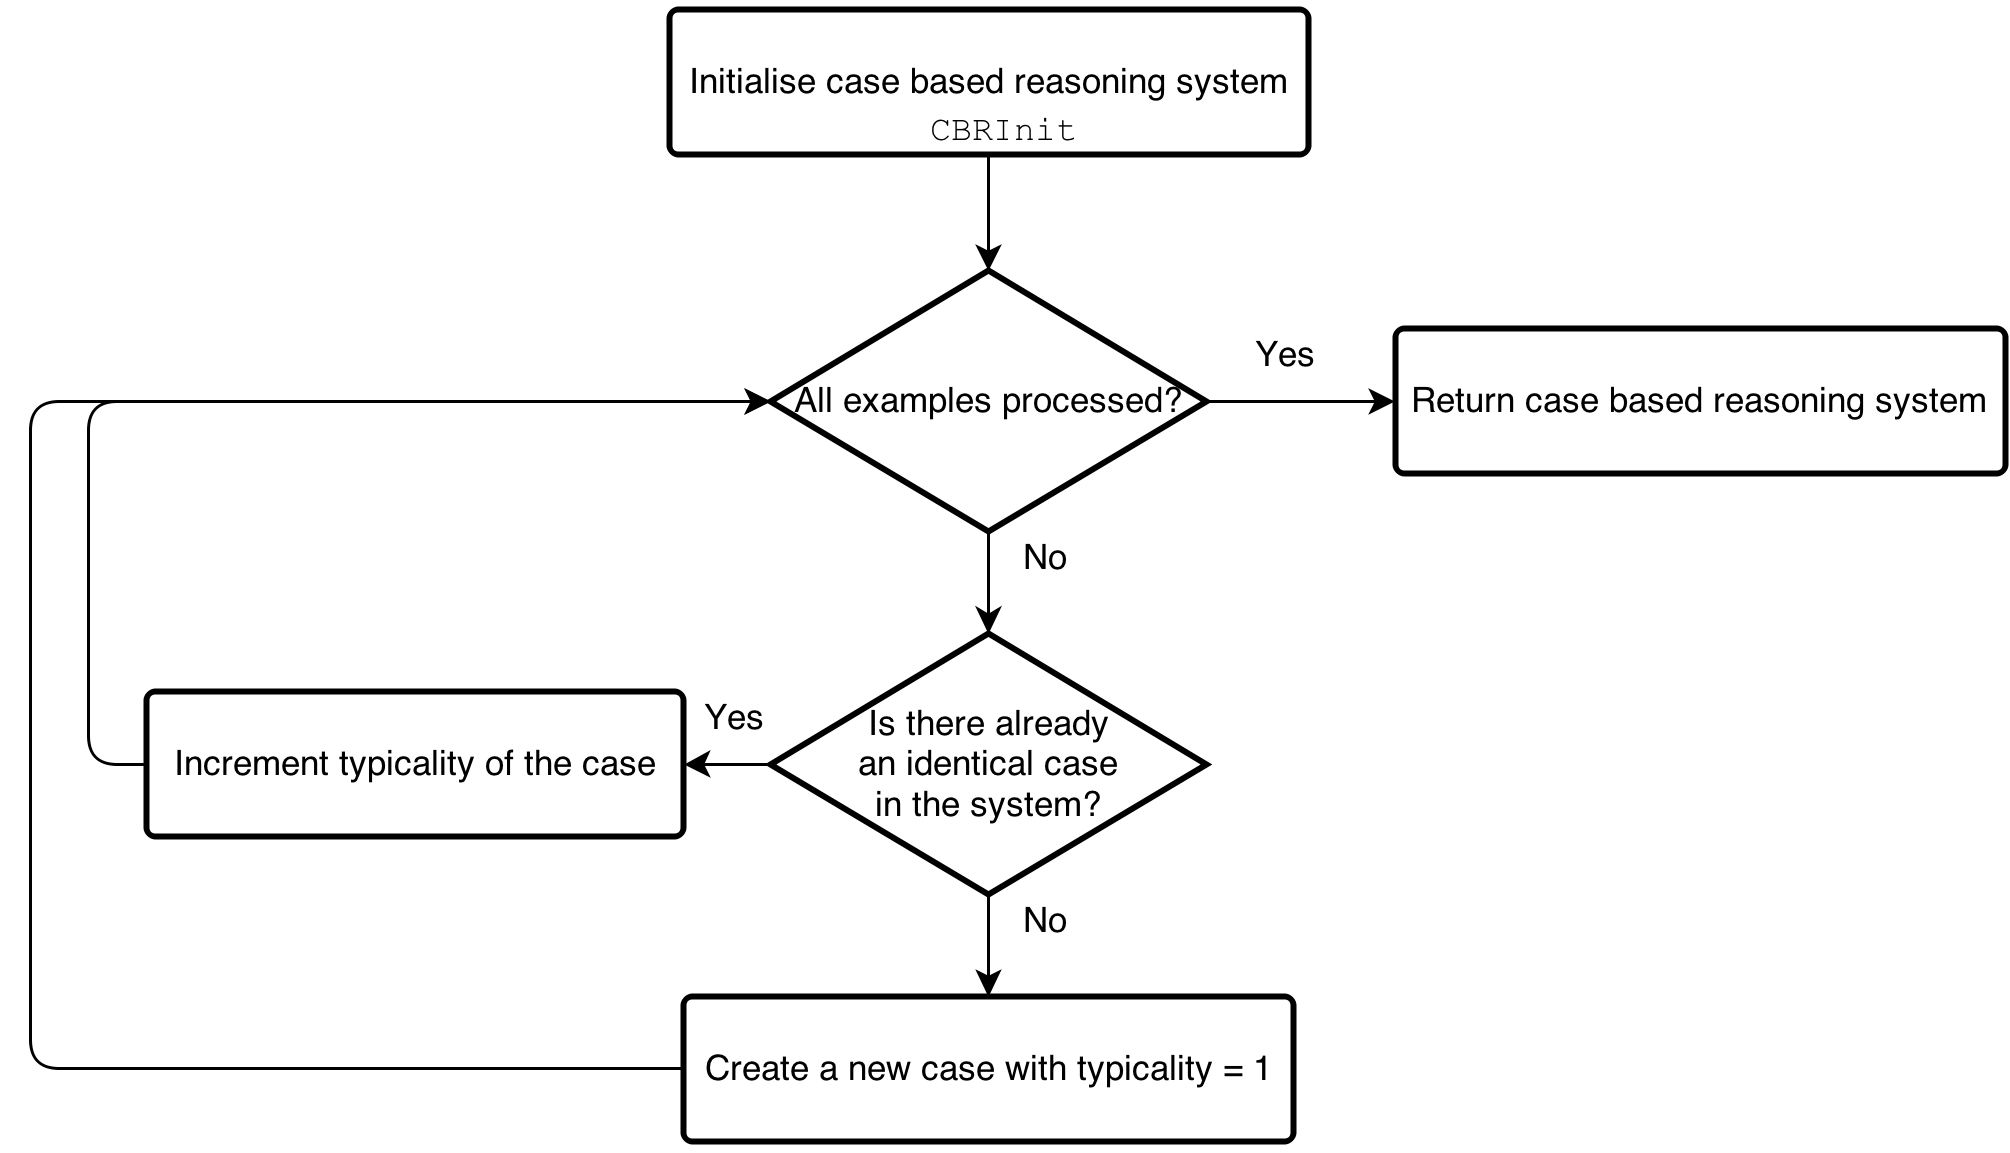
\includegraphics[width=0.9\columnwidth]{CBRInit}
\caption{Flowchart of the \texttt{CBRInit} function}
\label{flowchartCBRInit}
\end{figure}

\begin{figure}[H]
\center
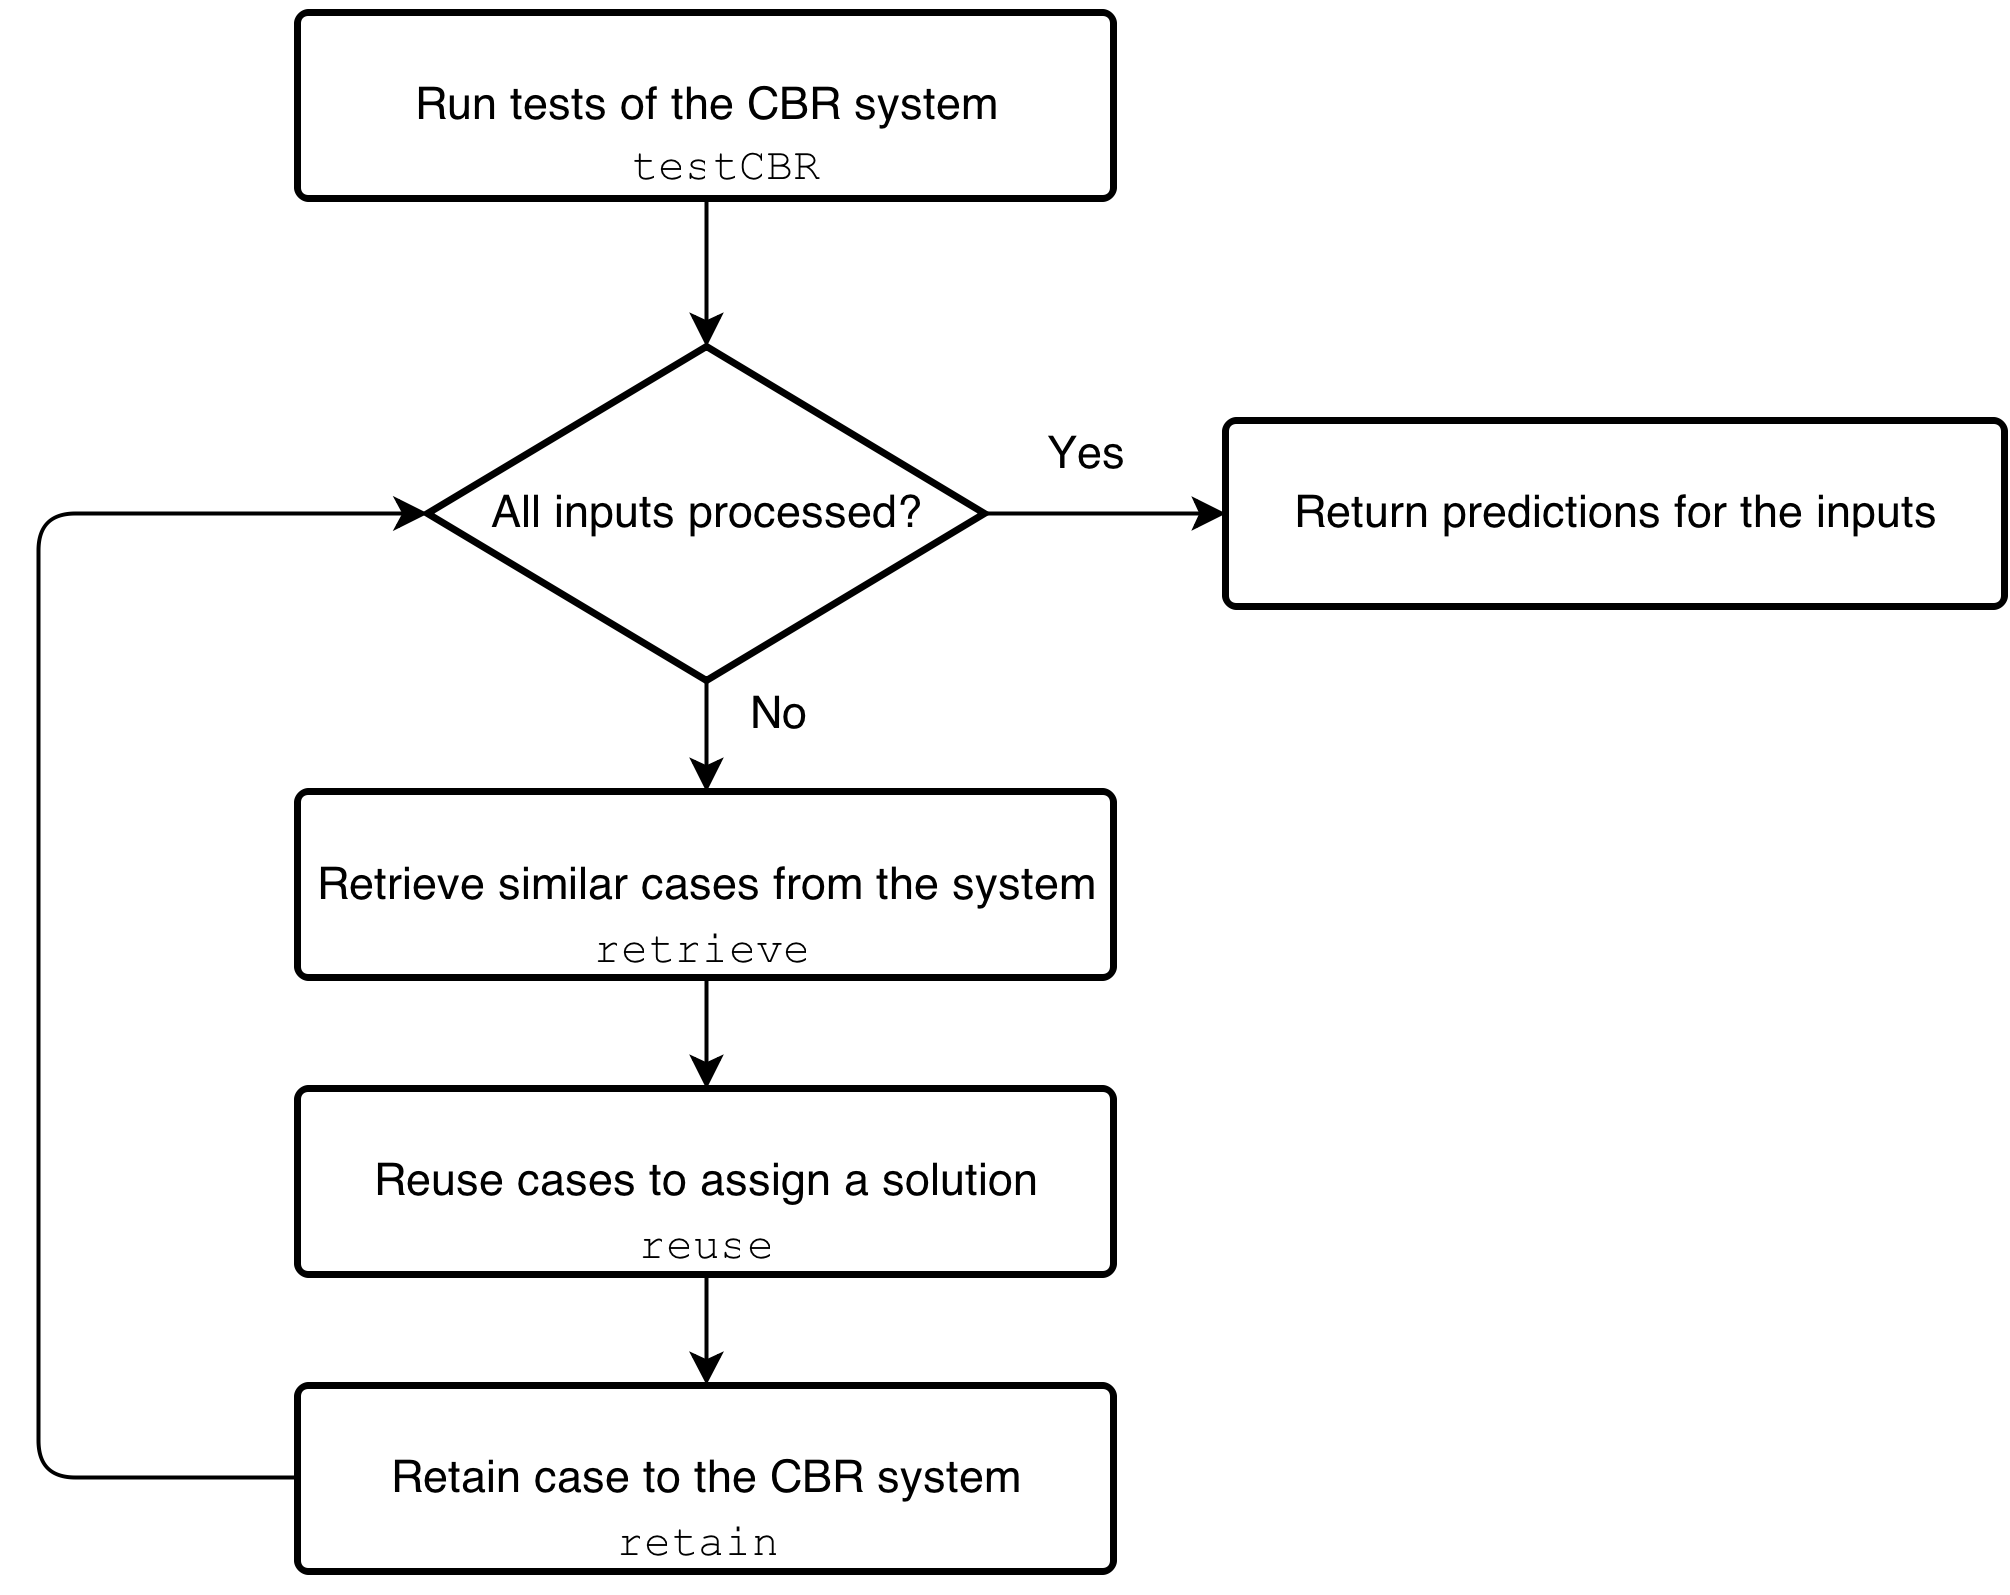
\includegraphics[width=0.9\columnwidth]{testCBR}
\caption{Flowchart of the \texttt{testCBR} function}
\label{flowchartTestCBR}
\end{figure}

\clearpage

%----------------------------------------------------------------------------------------

\end{document}